%%%%%%%%%%%%%%%%%%%%%%%%%%%%%%%%%%%%%%%%%%%%%%%%%%%%%%%%%%%%%%%%%%
%  = PREAMBLE =
% The preamble of a LaTeX document is the set of commands that 
%    precede the \begin{document} line.  It sets up the style of 
%    the document.
%%%%%%%%%%%%%%%%%%%%%%%%%%%%%%%%%%%%%%%%%%%%%%%%%%%%%%%%%%%%%%%%%%

\documentclass[aps,twocolumn, secnumarabic,balancelastpage,amsmath,amssymb,nofootinbib,floatfix]{revtex4-1}

\usepackage{graphicx}      % tools for importing graphics
\usepackage{tikz}
\usepackage{tikz-feynman}  % Requires TikZ-Feynman package
\usepackage{parskip}
\usepackage[colorlinks=true]{hyperref}  % this package should be added after 
                                        % all others.
                                        % usage: \url{http://web.mit.edu/8.13}

% \setlength{\parskip}{2pt}
\usetikzlibrary{decorations.pathmorphing}

%%%%%%%%%%%%%%%%%%%%%%%%%%%%%%%%%%%%%%%%%%%%%%%%%%%%%%%%%%%%%%%%%%%
% And now, begin the document...
%%%%%%%%%%%%%%%%%%%%%%%%%%%%%%%%%%%%%%%%%%%%%%%%%%%%%%%%%%%%%%%%%%%

\begin{document}

\title{Signal for a Higgs-like Particle of $124.22\pm1.16$ GeV from $H \to ZZ \to 4l$ Search}
% \author{Vinh Tran}
% \email{vinhtran@mit.edu}
\author{Yongao Hu}
\email{yongao@mit.edu}
\date{\today}
\affiliation{MIT Department of Physics}


\begin{abstract}
This report presents an excess in signal of a Higgs-like particle around 125 GeV in the $H \to ZZ \to 4l$ search. The data is collected from the 2011 and 2012 LHC run at $\sqrt{s} = 7$ TeV and $8$ TeV respectively. The results are consistent with the Standard Model prediction of a Higgs-like particle with a mass of $124.22\pm1.16$ GeV, with a significance of 2.4 $\sigma$. The discovery of Higgs boson completes the Standard Model of particle physics and confirms the Higgs mechanism. 
\end{abstract}

\maketitle

\section{Introduction}
Higgs boson and the corresponding Higgs mechanism are the key components of the Standard Model of particle physics (SM) \cite{PeskinSchroeder1995}. The Higgs boson is responsible for giving masses to SM particles \cite{PDG2023Higgs,PeskinSchroeder1995}. The discovery of the Higgs boson at the Large Hadron Collider (LHC) in 2012 is considered one of the most important achievements in particle physics in the past decade \cite{CMS:2012qbp}. This paper aims to reproduce the $H \to ZZ$ search in \cite{CMS:2012qbp} and analyze the data collected by CMS experiment from the 2011 and 2012 LHC run at $\sqrt{s} = 7$ TeV and $8$ TeV respectively to search for a Higgs-like particle with a mass of 125 GeV. 

\section{Theoretical Background}
\subsection{Higgs Bosons}
Higgs boson, a spin-0 massive particle, is a key component of SM. The corresponding Higgs field is a scalar field that permeates all of spacetime, and its non-zero vacuum expectation value (vev) leads to electroweak symmetry breaking, which gives masses to the W and Z bosons \cite{PeskinSchroeder1995, Weinberg1995}. Chiral fermions such as the matter content in SM also acquire mass through their interaction with the Higgs field \cite{PeskinSchroeder1995, Weinberg1995}. Up until 2010s, Higgs boson has not been observed. 

The Higgs boson is produced in high-energy collisions, such as those at the LHC \cite{CMS:2012qbp}. The decay channels of the Higgs boson include H$\rightarrow$ZZ, H$\rightarrow$WW, H$\rightarrow$bb, and H$\rightarrow$$\tau\tau$ \cite{Gunion:1990,PDG2023Higgs}. 

\subsection{H$\rightarrow$ZZ Decay}
The decay of the Higgs boson into two Z bosons ($H\to ZZ$) is a rare process, with a branching ratio of about 2.5\% for a Higgs boson mass of 125 GeV \cite{PDG2023Higgs}. The decay products of the Z bosons can be reconstructed from their decay into four leptons (pairs of $e^+e^-$ and/or $\mu^+\mu^-$). The final state consists of four charged leptons, which can be used to reconstruct the mass of the Higgs boson. The decay of the Z bosons into two charged leptons ($Z\rightarrow ll$) provides a clean signature for the Higgs boson search. This is because the products are non-hadronic, avoiding jet and hadronization modeling, and there are no neutrino produced, i.e. no missing signals. The mass of the Higgs boson can be reconstructed from the invariant mass of the four-lepton system. 

\begin{figure}[h]
  \begin{tikzpicture}[scale = 0.8]
    \begin{feynman}
      
        % -- Gluon emission vertices
        \vertex (g1) at (-1.2,  1) {\(g\)};
        \vertex (g2) at (-1.2, -1) {\(g\)};
      
        % -- Three vertices for the top/bottom quark loop (forming a triangle)
        \vertex (loop1) at (0,  0.8);
        \vertex (loop2) at (0, -0.8);
        \vertex (loop3) at (1,  0.0);
      
        % -- Higgs
        \vertex [right=2cm of loop3] (h);
      
        % -- Z bosons
        \vertex [right=2cm of h, yshift= 1.2cm] (z1);
        \vertex [right=2cm of h, yshift=-1.2cm] (z2);
      
        % -- Final leptons from the two Z decays
        \vertex [right=2cm of z1,  yshift= 0.7cm] (l1) {\(\ell^+\)};
        \vertex [right=2cm of z1,  yshift=-0.7cm] (l2) {\(\ell^-\)};
        \vertex [right=2cm of z2,  yshift= 0.7cm] (l3) {\(\ell^+\)};
        \vertex [right=2cm of z2,  yshift=-0.7cm] (l4) {\(\ell^-\)};
      
        % -- Define the diagram
        \diagram*{
          % Incoming protons -> gluons
          (g1) -- [gluon] (loop1),
          (g2) -- [gluon] (loop2),
      
          % The triangular loop (top or bottom quarks)
          (loop1) -- [fermion, edge label=\(q\)] (loop3),
          (loop3) -- [fermion, edge label=\(q\)] (loop2),
          (loop2) -- [fermion, edge label=\(q\)] (loop1),
      
          % Loop emits the Higgs
          (loop3) -- [scalar, edge label=\(h\)] (h),
      
          % Higgs decays into two Z bosons
          (h) -- [boson, edge label=\(Z\)] (z1),
          (h) -- [boson, edge label'=\(Z\)] (z2),
      
          % Each Z -> lepton pair
          (z1) -- [fermion]      (l1),
          (z1) -- [anti fermion] (l2),
          (z2) -- [fermion]      (l3),
          (z2) -- [anti fermion] (l4),
        };
      \end{feynman}
    \end{tikzpicture}
    \caption{Feynman diagram for the Higgs boson decay into two Z bosons and 4 leptons. The gluon fusion process is shown, where the Higgs boson is produced through a top or bottom quark loop. The gluons are produced when two protons collide with each other.}
  \label{fig:higgs}
  \end{figure}

  \section{Background Events}
Nevertheless, there are several background processes that are irreduccible, meaning that they mimic the signal and cannot be completely removed by selection criteria. 
The largest background is the continuum $ZZ^*$ production \cite{CMS:2012qbp}. Some of the production processes of $ZZ^*$ are shown in Figure \ref{fig:zz}. The continuum $ZZ^*$ production produces a pair of Z bosons from the annihilation of quarks and antiquarks or gluon-gluon fusion. 

\begin{figure*}[htbp]
    \centering
    %------------------ First Row: (a), (b), (c) ------------------%
    \begin{minipage}{0.32\textwidth}
        \centering
        %%%%%%%%%%%%%%%%%%%%%%%%%%%%%%%%%%%%%%%%%%%%%%%%%%%%%%%%
        % (a) qq -> ZZ via s-channel gamma*/Z*
        %%%%%%%%%%%%%%%%%%%%%%%%%%%%%%%%%%%%%%%%%%%%%%%%%%%%%%%%
        \begin{tikzpicture}
          \begin{feynman}
            % Define vertices
            \vertex (q1) at (-1,  0.8) {\(q\)};
            \vertex (q2) at (-1, -0.8) {\(q\)};
            \vertex (v)  at (0, 0);
            \vertex (w)  at (1, 0);
            \vertex (Z1) at (2,  0.8) {\(Z\)};
            \vertex (Z2) at (2, -0.8) {\(Z\)};

            % Diagram connections
            \diagram*{
              (q1) -- [fermion] (v) -- [fermion] (q2),
              (v) -- [boson, edge label = $\gamma / Z$] (w),
              (w) -- [boson] (Z1),
              (w) -- [boson] (Z2),
            };
          \end{feynman}
          % Label for diagram (a)
          \node at (0.5, -1.5) {(\textbf{a}) $qq \to \gamma^*/Z^* \to ZZ$};
        \end{tikzpicture}
    \end{minipage}
    \begin{minipage}{0.32\textwidth}
        \centering
        %%%%%%%%%%%%%%%%%%%%%%%%%%%%%%%%%%%%%%%%%%%%%%%%%%%%%%%%
        % (b) qq -> ZZ via t-channel quark exchange
        %%%%%%%%%%%%%%%%%%%%%%%%%%%%%%%%%%%%%%%%%%%%%%%%%%%%%%%%
        \begin{tikzpicture}
          \begin{feynman}
            % Define vertices
            \vertex (q1) at (-1.5, 0.8) {\(q\)};
            \vertex (q2) at (-1.5,-0.8) {\(q\)};
            \vertex (v1) at (0,  0.8);
            \vertex (v2) at (0, -0.8);
            \vertex (Z1) at ( 1.5,  0.8) {\(Z\)};
            \vertex (Z2) at ( 1.5, -0.8) {\(Z\)};

            % Diagram connections
            \diagram*{
              (q1) -- [fermion] (v1) -- [boson] (Z1),
              (q2) -- [fermion] (v2) -- [boson] (Z2),
              (v1) -- [fermion, edge label=\(q\)] (v2),
            };
          \end{feynman}
          % Label for diagram (b)
          \node at (0.5, -1.5) {(\textbf{b}) $t$-channel quark exchange};
        \end{tikzpicture}
    \end{minipage}
    \begin{minipage}{0.32\textwidth}
        \centering
        %%%%%%%%%%%%%%%%%%%%%%%%%%%%%%%%%%%%%%%%%%%%%%%%%%%%%%%%
        % (c) qq -> ZZ via u-channel quark exchange
        %%%%%%%%%%%%%%%%%%%%%%%%%%%%%%%%%%%%%%%%%%%%%%%%%%%%%%%%
        \begin{tikzpicture}
          \begin{feynman}
            % Define vertices
            \vertex (q1) at (-1.5, 0.8) {\(q\)};
            \vertex (q2) at (-1.5,-0.8) {\(q\)};
            \vertex (v1) at (0,  0.8);
            \vertex (v2) at (0, -0.8);
            \vertex (Z1) at ( 1.5,  0.8) {\(Z\)};
            \vertex (Z2) at ( 1.5, -0.8) {\(Z\)};

            % Connect so that final Z lines are "crossed"
            \diagram*{
              (q1) -- [fermion] (v1) -- [boson] (Z2),
              (q2) -- [fermion] (v2) -- [boson] (Z1),
              (v1) -- [fermion, edge label=\(q\)] (v2),
            };
          \end{feynman}
          % Label for diagram (c)
          \node at (0.5, -1.5) {(\textbf{c}) $u$-channel quark exchange};
        \end{tikzpicture}
    \end{minipage}

    %------------------ Second Row: (d), (e) ------------------%
    \vspace{1em}

    \begin{minipage}{0.32\textwidth}
        \centering
        %%%%%%%%%%%%%%%%%%%%%%%%%%%%%%%%%%%%%%%%%%%%%%%%%%%%%%%%
        % (d) gg -> ZZ box diagram #1
        %%%%%%%%%%%%%%%%%%%%%%%%%%%%%%%%%%%%%%%%%%%%%%%%%%%%%%%%
        \begin{tikzpicture}
          \begin{feynman}
            % Vertices of the box
            \vertex (g1) at (-1, 1) {\(g\)};
            \vertex (v1) at ( 0, 1);
            \vertex (v2) at ( 1, 1);
            \vertex (g2) at (-1, 0) {\(g\)};
            
            \vertex (v3) at ( 0, 0);
            \vertex (v4) at ( 1, 0);

            % Z bosons on the right
            \vertex (Z1) at ( 2,  1) {\(Z\)};
            \vertex (Z2) at ( 2, 0) {\(Z\)};

            % Diagram
            \diagram*{
              (g1) -- [gluon] (v1) -- [fermion, edge label=\(q\)] (v2),
              (v2) -- [fermion, edge label=\(q\)] (v4),
              (v4) -- [fermion, edge label=\(q\)] (v3)-- [gluon] (g2),
              (v3) -- [fermion, edge label=\(q\)] (v1),
              (v2) -- [boson] (Z1),
              (v4) -- [boson] (Z2),
            };
          \end{feynman}
          % Label for diagram (d)
          \node at (0.5, -0.8) {(\textbf{d}) $gg \to ZZ$ box diagram};
        \end{tikzpicture}
    \end{minipage}
    \begin{minipage}{0.32\textwidth}
        \centering
        %%%%%%%%%%%%%%%%%%%%%%%%%%%%%%%%%%%%%%%%%%%%%%%%%%%%%%%%
        % (e) gg -> ZZ box diagram #2 (crossed)
        %%%%%%%%%%%%%%%%%%%%%%%%%%%%%%%%%%%%%%%%%%%%%%%%%%%%%%%%
        \begin{tikzpicture}
          \begin{feynman}
            % Vertices of the box
            \vertex (g1) at (-1, 1) {\(g\)};
            \vertex (v1) at ( 0, 1);
            \vertex (v2) at ( 1, 1);
            \vertex (g2) at (-1, 0) {\(g\)};
            
            \vertex (v3) at ( 0, 0);
            \vertex (v4) at ( 1, 0);

            % Z bosons on the right
            \vertex (Z1) at ( 2,  1) {\(Z\)};
            \vertex (Z2) at ( 2, 0) {\(Z\)};

            % Diagram
            \diagram*{
              (g1) -- [gluon] (v1) -- [fermion, edge label=\(q\)] (v2),
              (v2) -- [fermion, edge label=\(q\)] (v4),
              (v4) -- [fermion, edge label=\(q\)] (v3)-- [gluon] (g2),
              (v3) -- [fermion, edge label=\(q\)] (v1),
              (v2) -- [boson] (Z2),
              (v4) -- [boson] (Z1),
            };
          \end{feynman}
          % Label for diagram (e)
          \node at (1, -0.8) {(\textbf{e}) $gg \to ZZ$ box diagram (crossed)};
        \end{tikzpicture}
    \end{minipage}
    \caption{Representative Feynman diagrams for continuum $ZZ^*$ production:
             (a)–(c) from quark–antiquark initial state,
             (d)–(e) from gluon–gluon initial state.}
    \label{fig:zz}
\end{figure*}

Besides, there are additional backgrounds from the production from Z+jets production that produces two isolated leptons, and $t\bar{t}$ production, the pair production of top and anti-top quarks that decays into leptons \cite{Hu2020HiggsTo4L}. These processes can also produce events that are irreduccible and resemble signals, but they are less significant than the continuum ZZ* production. 


\section{Experimental Background}
LHC is a proton-proton collider located at CERN, Geneva, Switzerland \cite{CMS:2012qbp}. The LHC is the largest and most powerful particle accelerator in the world, with a design energy of 14 TeV \cite{CMS:2012qbp}. The CMS experiment is a general-purpose detector designed to study a wide range of physics processes, including Higgs boson searches. Here, we are using the Run 1 data with center-of-mass energy $\sqrt{s} = 7$ TeV (in 2011) and $8$ TeV (in 2012) \cite{CMS_2010_data,MIT:Higgs4L2020,Hu2020HiggsTo4L,CMS:2012qbp}.

\subsection{CMS Detector}
CMS experiment includes a superconducting solenoid that provides a magnetic field of 3.8 T to bend the trajectories of charged particles, a silicon tracker to measure the momenta of charged particles, a lead tungstate crystal electromagnetic calorimeter (ECAL) to measure the energy of photons and electrons, a brass/scintillator hadron calorimeter (HCAL) to measure the energy of hadrons, and gas-ionization muon detectors \cite{CMS:2012qbp}. 

Pseudorapidity $\eta$ is used to describe the angular distribution of particles in the CMS detector. Pseudorapidity is defined as $\eta=-\ln(\tan(\frac{\theta}{2}))$, where $\theta$ is the polar angle from the positive $z$-axis. The silicon tracker tracks charged particles within the pseudorapidity range of $|\eta| < 2.5$. The ECAL and HCAL measures particles within the pseudorapidity range of $|\eta| < 3.0$. The muon detectors detect muons within the pseudorapidity range of $|\eta| < 2.4$ \cite{CMS:2012qbp}. 


\subsection{Monte Carlo Simulation}
The signal and background processes are generated using monte carlo simulation. First, the underlying hard-scattering processes are generated with \textsc{POWHEG} \cite{Alioli:2010xd} or \textsc{MadGraph}4 \cite{Alwall:2007st}, followed by parton showering and hadronization using \textsc{PYTHIA}6.4 \cite{Sjostrand:2006za}. The resulting events are then passed through a \textsc{GEANT4}-based \cite{Agostinelli:2002hh} simulation of the detector. The parton distribution functions (PDFs) are chosen according to \textsc{PDF4LHC} working group recommendations \cite{Botje:2011sn,Alekhin:2011sk,Lai:2010vv,Ball:2011mu}. The simulation data utilized in this study is obtained from CMS Open Data \cite{CMS_2010_data,MIT:Higgs4L2020,Hu2020HiggsTo4L}.

\section{Selection Criteria}

\subsection{Preliminary Selection}
The data from \cite{MIT:Higgs4L2020,Hu2020HiggsTo4L} has been pre-processed to remove the events that do not pass the preliminary selection criteria. The events are selected based on the following criteria \cite{Hu2020HiggsTo4L}:

\begin{itemize}
  \item The events contains only four leptons, which are either electrons or muons as the final state particles.
  \item Transverse impact parameter with respect to the primary vertex $|d_{xy}| < 0.5\;\text{cm}$.
  \item Longitudinal impact parameter with respect to primary vertex $|d_{z}| < 1\;\text{cm}$.
  \item 3D impact parameter significance: $|\text{SIP}| < 4$, where $\text{SIP} = \frac{I}{\sigma_I}$, $I$ is the 3D lepton impact parameter, and $\sigma_I$ is its uncertainty. This ensures that the lepton pairs from Z boson decays originate from the same primary vertex.
  \item Muon and electron selection criteria: relative isolation of the lepton (reIso), the scalar sum of the transverse momenta of particles reconstructed within a distance $\Delta R$ of the object, normalized to the $p_T$ of the object, is smaller than 0.4 within a cone $\Delta R = 0.4$, where $\Delta R = \sqrt{(\Delta\eta)^2 + (\Delta\phi)^2}$. $\Delta \eta$ is the difference in pseudorapidity, and $\Delta \phi$ is the difference in azimuthal angle. 
\end{itemize}

We further apply the following selection criteria to select the events that pass the preliminary selection \cite{CMS:2012qbp}:
\begin{itemize}
  \item Pseudorapidity of the lepton: $|\eta_e| < 2.5$ for electrons, $|\eta_\mu| < 2.4$ for muons.
  \item Transverse momentum of the lepton: $p_T > 20\;\text{GeV}$ for electrons, $p_T > 10\;\text{GeV}$ for muons.
  \item The four-lepton system includes two pairs of same-flavor opposite-charged leptons are required to form the four-lepton system. 
  \item The pair of leptons with invariant mass closer to mass of Z boson have mass between $40\;\text{GeV}$ and $120\;\text{GeV}$, and the other pair have mass between $12\;\text{GeV}$ and $120\;\text{GeV}$.
\end{itemize}

\subsection{Neural Network}
The neural network (NN) is used to classify the events into signal and background, trained using the pre-processed data. The NN utilizes fully‑connected Graph Convolutional Network (GCN) \cite{kipf2017semi} with each lepton as a node and \textsc{PyTorch} backend \cite{paszke2019pytorch}. The input features of the NN are the $x$ and $y$ components of momenta, and particle ID of the four-lepton system of the Monte Carlo simulation with invariant mass between 100 GeV and 160 GeV. We did not use the $z$ component of momenta or the mass of the particles because otherwise the NN can reconstruct the invariant mass and use that as the primary feature. 

We use 72\% of the data for training, 18\% of the data for validation, and 10\% of the data for testing. Each lepton is processed individually with three layers of size 32 each. The network aggregates information symmetrically across all leptons. Once the 4 leptons are combined, we have more fully-connected layers (256 $\to$ 64 $\to$ 16 $\to$ 4) before the final output. The output is yes/no for signal/background. 

The NN is trained using the Adam optimizer \cite{kingma2014adam} with a learning rate of $3\times10^{-4}$. The loss function is binary cross-entropy \cite{goodfellow2016deep}. The NN is trained for 100 epochs. The NN is trained to minimize the loss function, and the accuracy is calculated as the number of correct predictions divided by the total number of predictions. The training and validation loss and validation accuracy are shown in Figure \ref{fig:accuracy}. 
\begin{figure}[h]
  \centering
  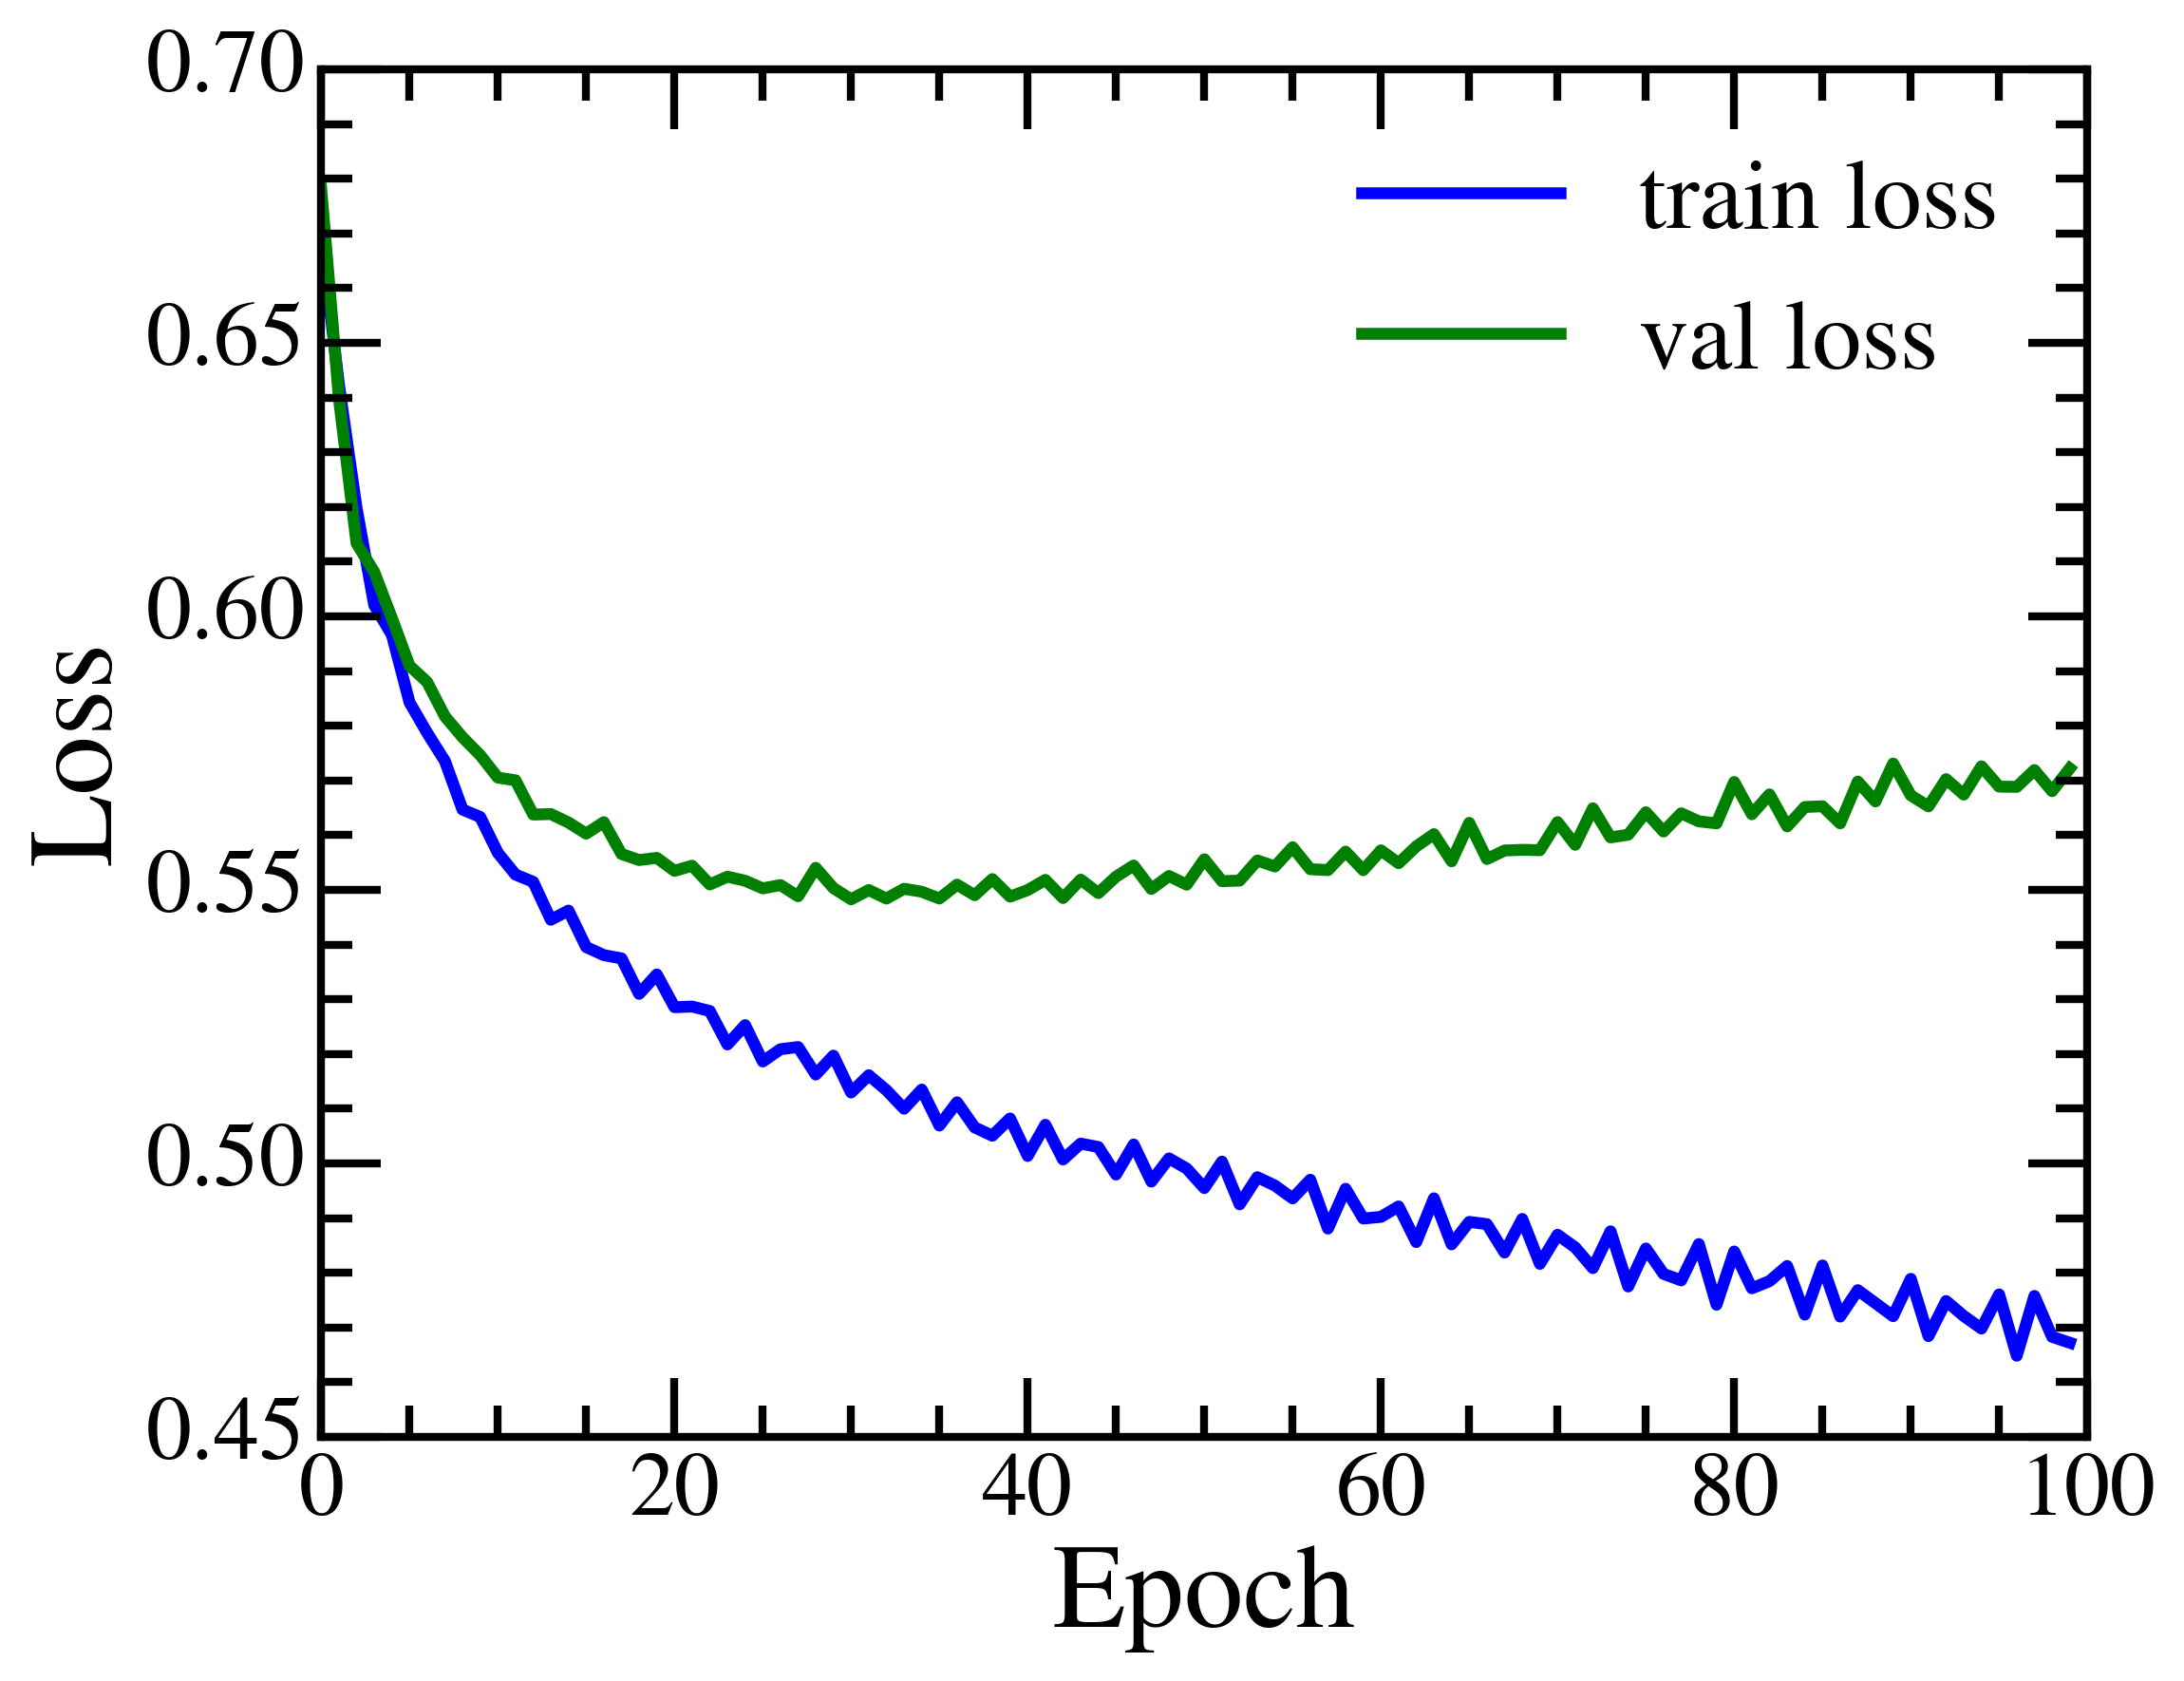
\includegraphics[width=0.23\textwidth]{Figures/training_loss.png}
  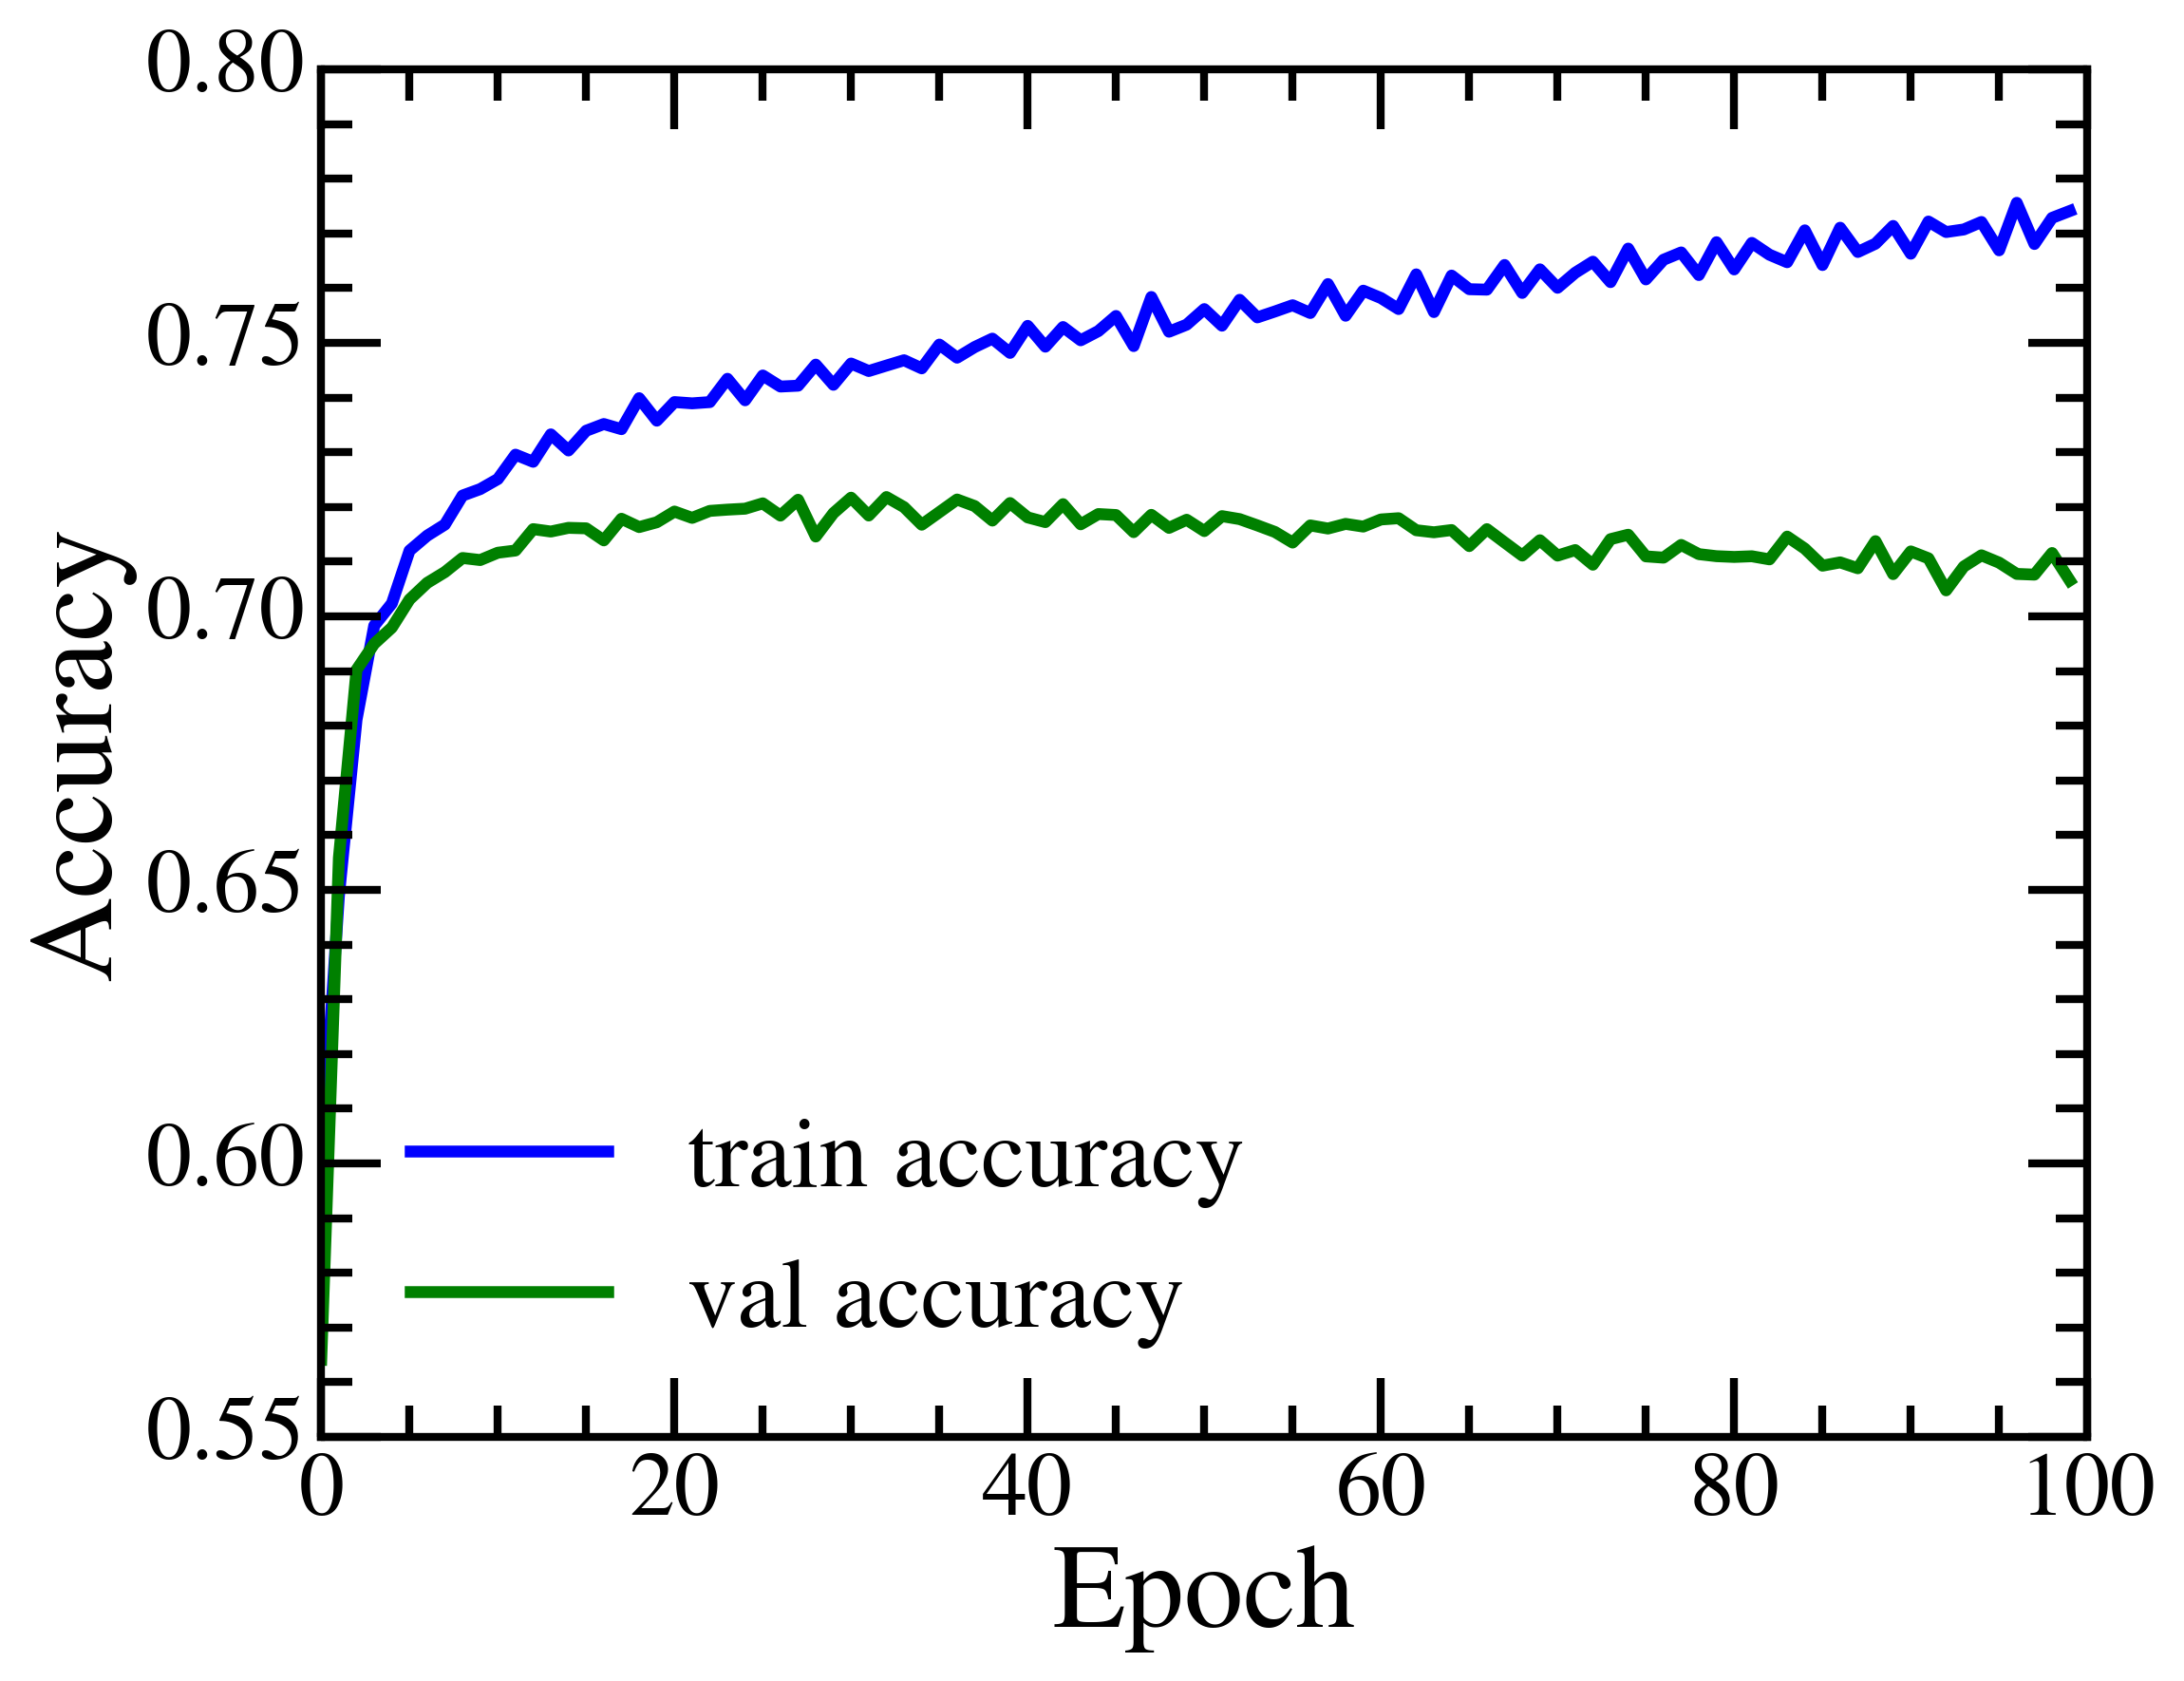
\includegraphics[width=0.23\textwidth]{Figures/training_accuracy.png}
  \caption{Training and validation loss and accuracy of the neural network. The loss is calculated using binary cross-entropy. The accuracy is calculated as the number of correct predictions divided by the total number of predictions.}
  \label{fig:accuracy}
\end{figure}

\subsection{Result}

After applying the NN and the selection criteria to the monte-carlo simulation and data, we obtain the final dataset, shown in Figure \ref{fig:dataset}. The dataset is used to calculate the significance of the excess in signal as a function of mass. 

\begin{figure}[h]
  \centering
  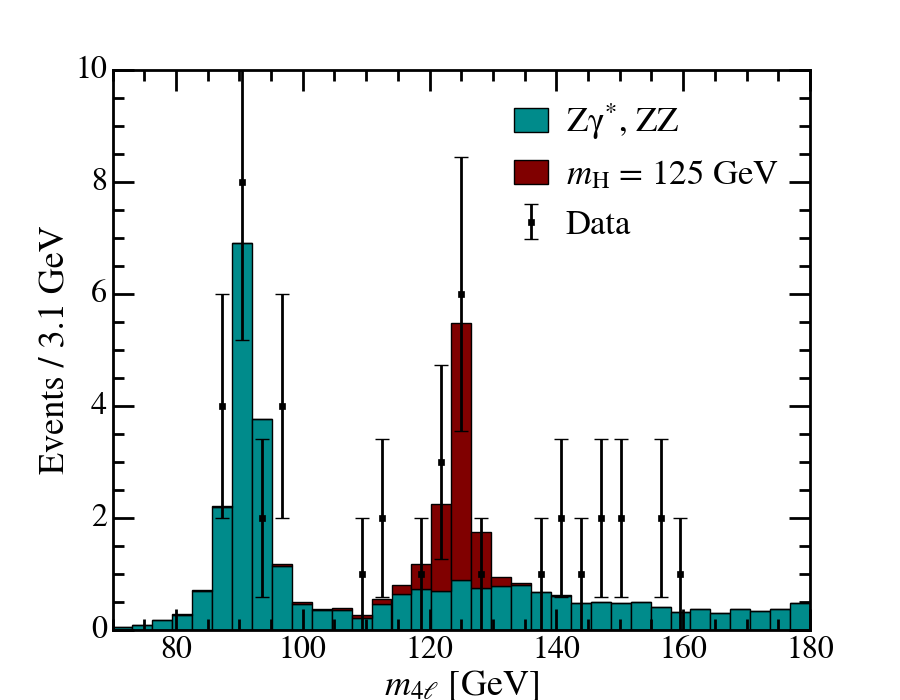
\includegraphics[width=0.45\textwidth]{Figures/data.png}
  \caption{Final dataset after applying the selection criteria and the neural network. The error bar comes from the standard statistical uncertainty of the data.}
  \label{fig:dataset}
\end{figure}


\section{Statistical Analysis}
The statistical analysis is performed using the profile likelihood ratio test \cite{Cowan:2010js}. We have two hypotheses: the null hypothesis (H0) and the alternative hypothesis (H1). The null hypothesis is that there is no signal (background only), and the alternative hypothesis is that there is a signal (signal and background). We approximate the signal as a Gaussian distribution on top of the background. 


We can calculate the p-value of the data using the likelihood ratio test statistic. We use $\chi^2$ fitting to fit the data to the background-only hypothesis (H0) and the signal-plus-background hypothesis (H1). H0 has 1 degree of freedom (scaling of background) while H1 has 4 degrees of freedom (scaling of background, signal strength, signal width, higgs mass). We can then compute the p-value from the difference of the two reduced $\chi^2$ values:
\begin{equation}
  p = 1 - F_{\chi^2_{\Delta \nu}}(\Delta \chi^2)
\end{equation}
where $F_{\chi^2_{\nu}}$ is the cumulative distribution function of the $\chi^2$ distribution with $\nu$ degrees of freedom, $\Delta \chi^2 = \chi^2_{H0} - \chi^2_{H1}$ is the difference of the two reduced $\chi^2$ values, and $\Delta\nu$ is the difference in degrees of freedom between the two hypotheses. 

The result is shown in Figure \ref{fig:likelihood}. 
\begin{figure}[h]
  \centering
  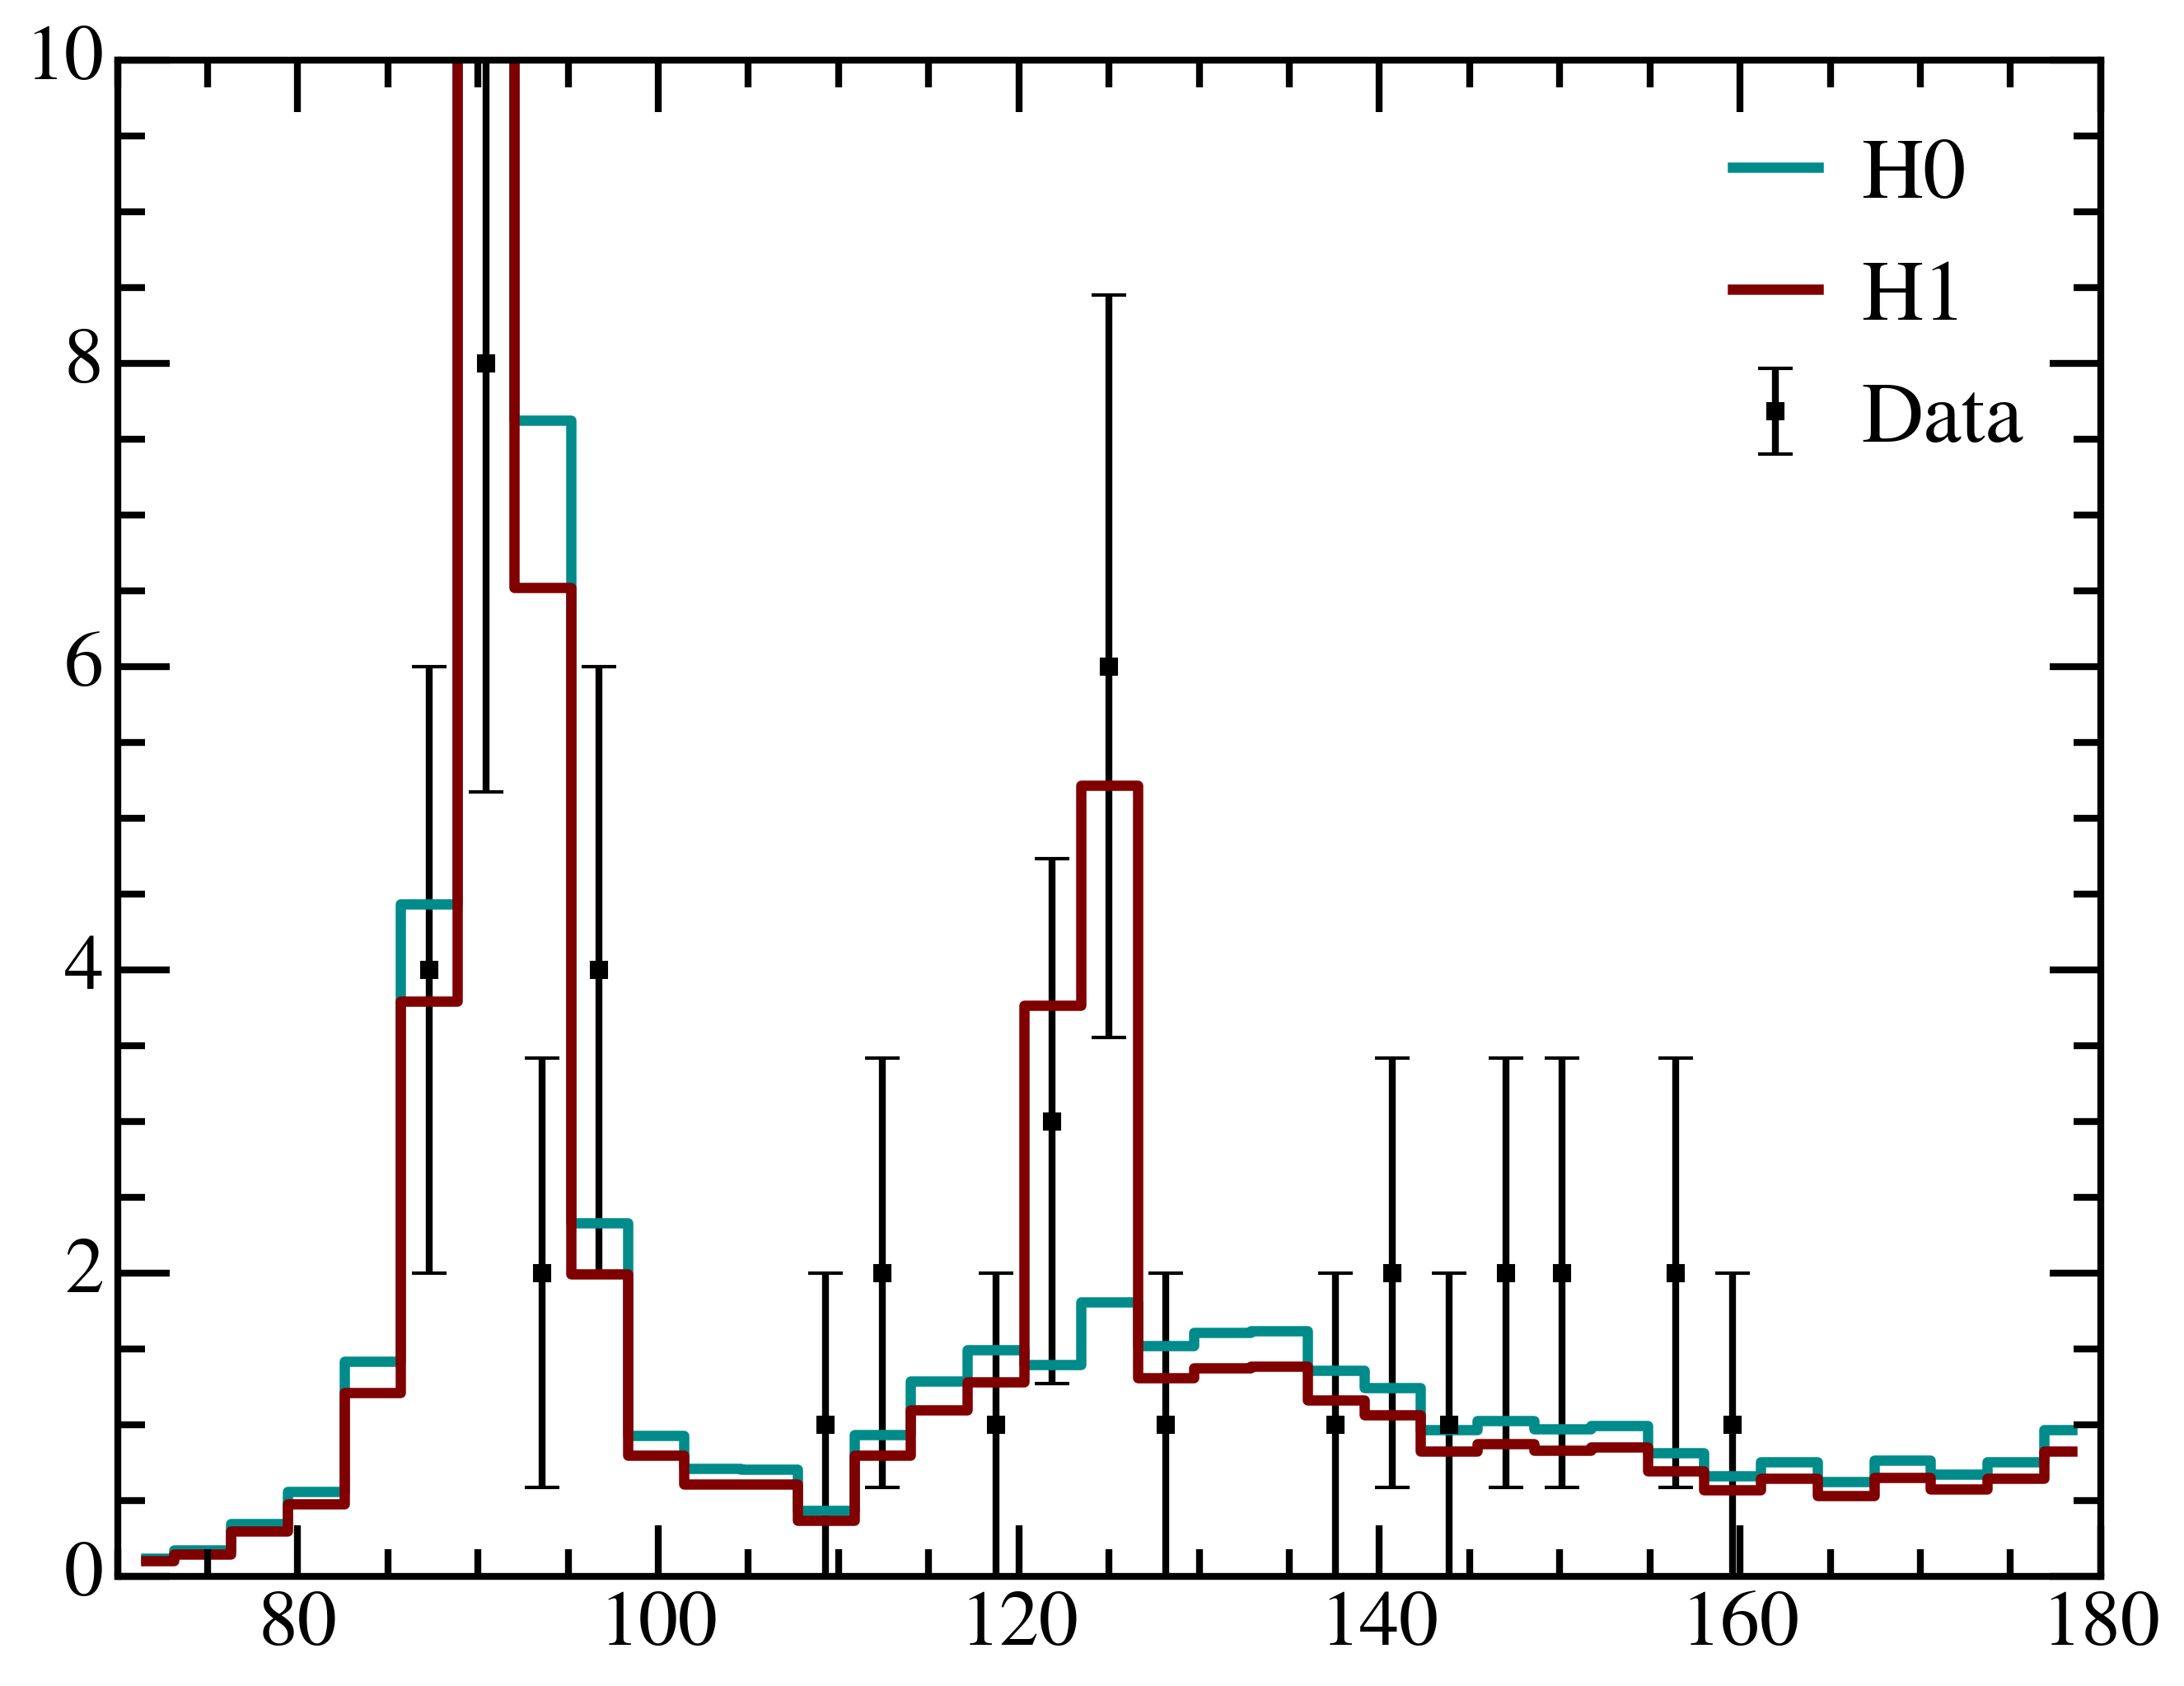
\includegraphics[width=0.45\textwidth]{Figures/hypo_testing.png}
  \caption{Sample H0 and H1 likelihood distributions for $m_h=125\text{ GeV}$. The blue line indicates the null hypothesis, and the red line indicates the alternative hypothesis.}
  \label{fig:likelihood}
\end{figure}

The p-value is then used to calculate the significance of the excess, the number of standard deviations away from the null hypothesis, in signal according to the formula \cite{Cowan:2010js}:
\begin{equation}
  Z = \Phi^{-1}(1 - p) = \sqrt{2} \text{erf}^{-1}(1 - 2p)
\end{equation}
where $\Phi^{-1}$ is the inverse cumulative distribution function of the standard normal distribution, and $\text{erf}^{-1}$ is the inverse error function. The significance is then used to determine whether the excess in signal is statistically significant.

We scanned mass range from 110 GeV to 160 GeV and different width of the Higgs peak by approximating the signal as a Gaussian distribution on top of the background. We then performed statistical hypothesis testing using the profile likelihood ratio test to determine the significance of the excess in signal at each mass point. The results are shown in Figure \ref{fig:significance}. A pronounced minimum in the $p$-value distribution occurs at
\[
  m_H \simeq 123.8\ \mathrm{GeV}, 
  \; p = 0.016,
  \;\text{(local significance}\approx2.4\sigma\text{)}.
\]
The $p$-value remains essentially unchanged under variations of the standard deviation $\sigma_{m_H}$, indicating that the signal is insensitive to the Gaussian peak width. To obtain a more accurate determination of the Higgs mass and its uncertainty, we apply a bootstrap resampling: the observed event counts are fluctuated within their uncertainties and the analysis is repeated on each resampled dataset. From this procedure we find
\[
  m_H = 124.22 \pm 1.16\ \mathrm{GeV},
\]
in good agreement with the expected value $m_H\simeq125\,$GeV in the CMS paper \cite{CMS:2012qbp}. 

\begin{figure}[h]
  \centering
  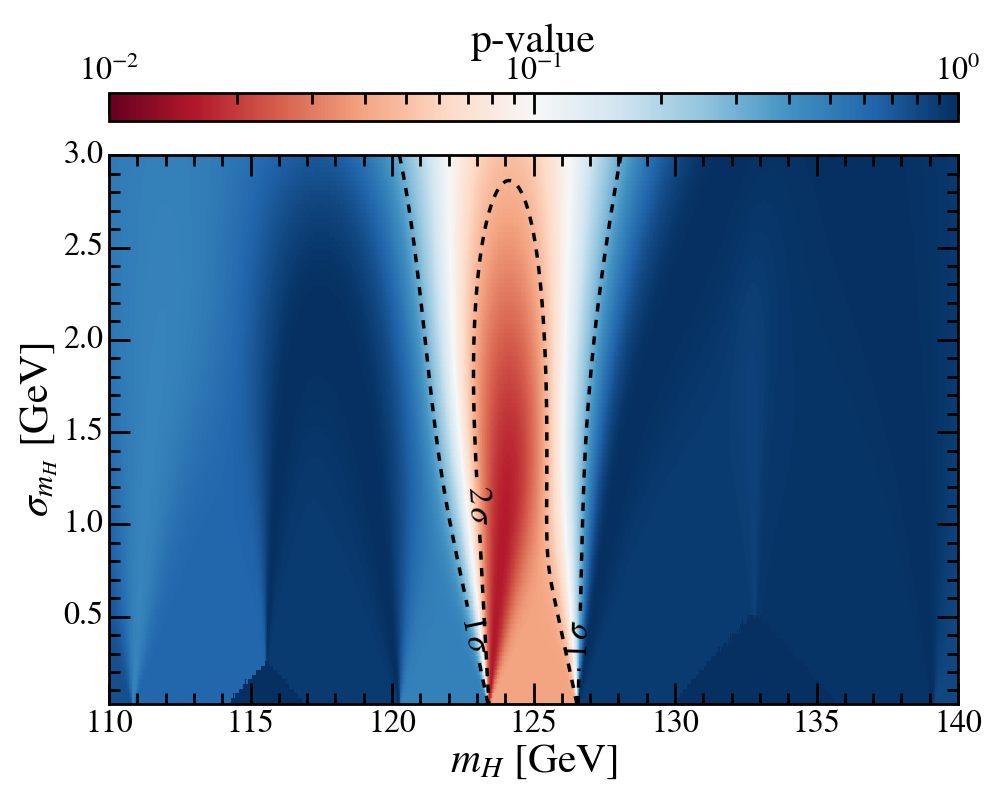
\includegraphics[width=0.45\textwidth]{Figures/p-value-2.png}
  \caption{Significance of the excess in signal as a function of mass and width of peak. The profile of the $p$-value is mapped over the Higgs boson mass $m_H$ and the signal peak's standard deviation $\sigma_{m_H}$.  In the contour plot, dashed lines mark the regions of local significance at the 1$\sigma$ and 2$\sigma$ levels. Each regression fit holds $\sigma_{m_H}$ fixed, but the overall hypothesis test treats $\sigma_{m_H}$ as a free parameter.}
  \label{fig:significance}
\end{figure}


\subsection{Uncertainty Estimation}

The statistical uncertainty comes from the finite size of the events recorded, which is estimated using the standard deviation of the number of events in each bin. The statistical uncertainty can be improved by measuring more events for longer duration with a higher combined luminosity of the dataset, which LHC did in 2015 and 2016 in Run 2 \cite{ATLAS:2023oaq}. 

The major source of systematic uncertainty comes from the Monte Carlo simulation. In particular, the choice of parton distribution function (PDF) and the choice of the generator can affect the results. We used \textsc{PDF4LHC} working group recommendation \cite{Botje:2011sn,Alekhin:2011sk,Lai:2010vv,Ball:2011mu} for the choice of PDF. 

\section{Conclusion}
In conclusion, we have reproduced the analysis done in \cite{CMS:2012qbp} and found an excess in signal of a Higgs-like particle around 125 GeV in the $H \to ZZ \to 4l$ search. The results are consistent with the Standard Model prediction of a Higgs-like particle with a mass of $124.22\pm1.16$ GeV, with a significance of 2.4 $\sigma$. The discovery of Higgs boson completes the Standard Model of particle physics and confirms the Higgs mechanism, The results also provide a strong motivation for further studies of the Higgs boson and its properties, including its couplings to other particles, its role in electroweak symmetry breaking, and potentially more complicated Higgs sectors beyond the Standard Model.

\vfill\null

\begin{acknowledgments} The author gratefully acknowledges their lab partner V. Tran for their invaluable assistance. The author also thanks the 8.13 teaching team for their guidance in the lab. This work was supported by the MIT Department of Physics. 
\end{acknowledgments}

\bibliographystyle{abbrv}
\bibliography{ref}
\end{document}

